\documentclass{extbook}
\usepackage[papersize={8.5in,11in},top=1in,bottom=1in]{geometry}
\RequirePackage{fix-cm}
\usepackage[T1]{fontenc}
\usepackage{lmodern}
\usepackage{fullpage}
\usepackage{titlesec}
\usepackage{parskip}
\usepackage{float}
\usepackage{url}
\usepackage{hyperref}
\usepackage{graphicx}
\usepackage{tcolorbox}
\usepackage{tabularx}
\usepackage{xcolor}
\usepackage{titlesec}
\usepackage{amsmath}
\usepackage{tcolorbox}
\usepackage{tabularx}
\usepackage{listings}

\lstset
{
    breaklines=true,
    tabsize=3,
    showstringspaces=false
}

\lstdefinestyle{vbstyle}{
  language={[Visual]Basic},
  backgroundcolor=\color{lightgray}, % Color de fondo
  basicstyle=\ttfamily\small, % Tamanoo y tipo de fuente
  keywordstyle=\color{blue}, % Color para palabras clave
  commentstyle=\color{green}, % Color para comentarios
  stringstyle=\color{red}, % Ccadenas de texto
  numberstyle=\tiny\color{gray}, % Coñor y tamaño de los números de línea
  stepnumber=1,
  numbers=left, % esto es para el # de la linea
  numbersep=5pt,
  showstringspaces=false,
  frame=single,
  breaklines=true
}


\renewcommand{\contentsname}{Contenido}
\renewcommand{\figurename}{Figura}
\renewcommand{\listtablename}{Lista de tablas}
\renewcommand{\listfigurename}{Lista de figuras}
\usepackage[fontsize=13.5pt]{fontsize}
\setlength{\parindent}{0pt}

\titleformat{\chapter}[display]
  {\bfseries\huge} % Estilo del título
  {\hfill\Large} % Alineación a la derecha
  {3ex} % Espaciado entre el número del capítulo y el título
  {\vspace{-5cm}\titlerule\vspace{1.5ex}\hfill} % Regla arriba y alineación del título a la derecha
  [\vspace{1ex}\titlerule] % Regla debajo del título


  \makeatletter
  \patchcmd{\chapter}
    {\if@openright\cleardoublepage\else\clearpage\fi}
    {\clearpage}
    {}{}
  \makeatother

  \definecolor{codegreen}{rgb}{0,0.6,0}
  \definecolor{codegray}{rgb}{0.5,0.5,0.5}
  \definecolor{codepurple}{rgb}{0.58,0,0.82}
  \definecolor{backcolour}{rgb}{0.95,0.95,0.92}

\begin{document}
\begin{titlepage}
  \begin{center}
      {\huge \textbf{Universidad Tecnológica de Panamá}}\\
      \vspace{3mm}
      {\Large \textbf{Centro Regional De Veraguas}}

      \begin{figure}[H]
          \centering
          
\includegraphics[scale = 0.07]{Imagenes/utp.png}
          
\includegraphics[scale = 0.58]{Imagenes/fisc.png}
      \end{figure}
      {\Large \textbf{Facultad de Ingeniería de Sistemas Computacionales}}\\
      \vspace{5mm}
      
      {\Large \textbf{Curso: Herramientas de Programación Aplicada III}}\medskip
      
      {\Large \textbf{Profesora: Milka de Escobar}}

      \rule{\linewidth}{0.75mm}\\
          {\Large \textsc{Informe MenuStrip}} 
      \rule{\linewidth}{0.75mm}\medskip

      {\Large \textbf{Estudiantes}}\\
      \vspace{5mm}
      {\Large \textbf{Elbin Puga, Arland Barrera}}
      \vfill
      {\Huge \textbf{2024}}

  \end{center}
\end{titlepage}
\tableofcontents
\listoffigures
%\listoftables para lista de tablas 
\chapter{Introducción}
El MenuStrip en Visual Studio es una herramienta esencial para crear interfaces gráficas en aplicaciones de Windows Forms, permitiendo añadir menús desplegables de manera sencilla y eficiente. Estos menús proporcionan opciones organizadas que mejoran la usabilidad de las aplicaciones, como acceder a funciones, configuraciones o acciones específicas. Al ser altamente personalizable, el MenuStrip facilita la implementación de jerarquías de menús, accesos rápidos y atajos de teclado, contribuyendo a una mejor experiencia de usuario.
\chapter{Desarrollo}
\section{MenuStrip}
Para acceder a la herramienta \emph{MenuStrip} se selecciona la opción correspondiente en la \emph{ToolBox}.

\begin{figure}[H]
  \centering
  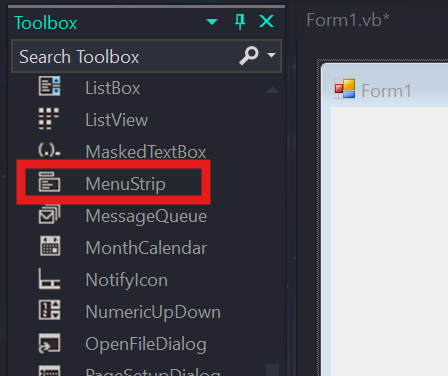
\includegraphics[scale = 1]{Imagenes/manual_1.png}
  \caption{Herramienta MenuStrip}{Fuente: Propia}
\end{figure}

En la ventana del \emph{Form} aparece en la parte superior el \emph{MenuStrip}.

\begin{figure}[H]
  \centering
  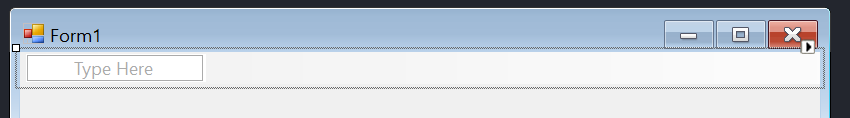
\includegraphics[scale = 0.7]{Imagenes/manual_2.png}
  \caption{MenuStrip en la ventana Form}{Fuente: Propia}
\end{figure}

Se puede inidcar el nombre del \emph{menú desplegable} y los \emph{submenús} que conforman la interfaz.

\begin{figure}[htb]
  \centering
  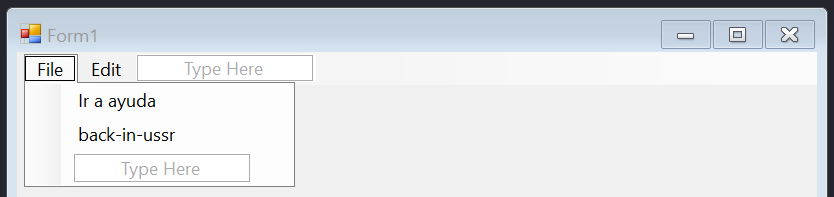
\includegraphics[scale = 0.6]{Imagenes/manual_3.png}
  \caption{Menú desplegable}{Fuente: Propia}
\end{figure}

Se puede programar la acción que ejecuta cada \emph{submenú} haciendo doble click izquierdo sobre el mismo.

\begin{figure}[htb]
  \centering
  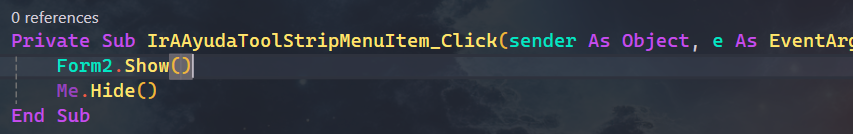
\includegraphics[scale = 0.6]{Imagenes/manual_4.png}
  \caption{Programación de submenú}{Fuente: Propia}
\end{figure}
\section{Programa de ejmeplo}
\subsection{Capturas de ejecución}
\begin{figure}[H]
  \centering
  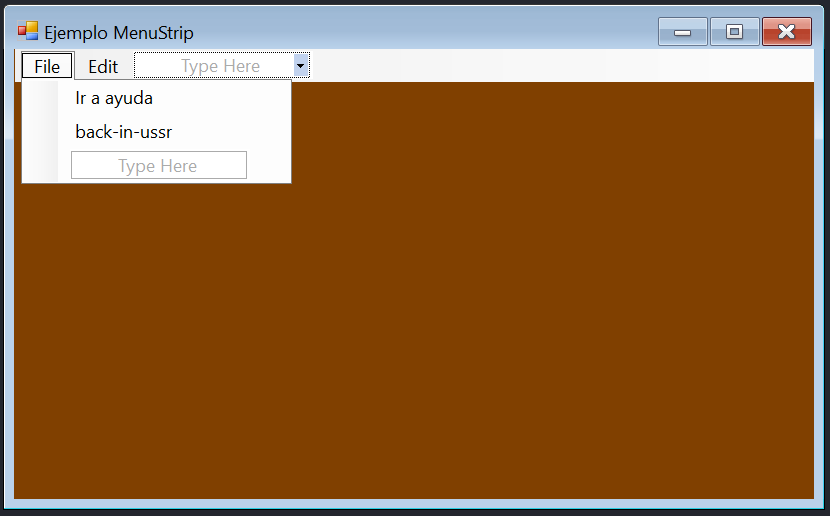
\includegraphics[scale = 0.5]{Imagenes/ui_1.png}
  \caption{Form 1}{Fuente: Propia}
\end{figure}

\begin{figure}[htb]
  \centering
  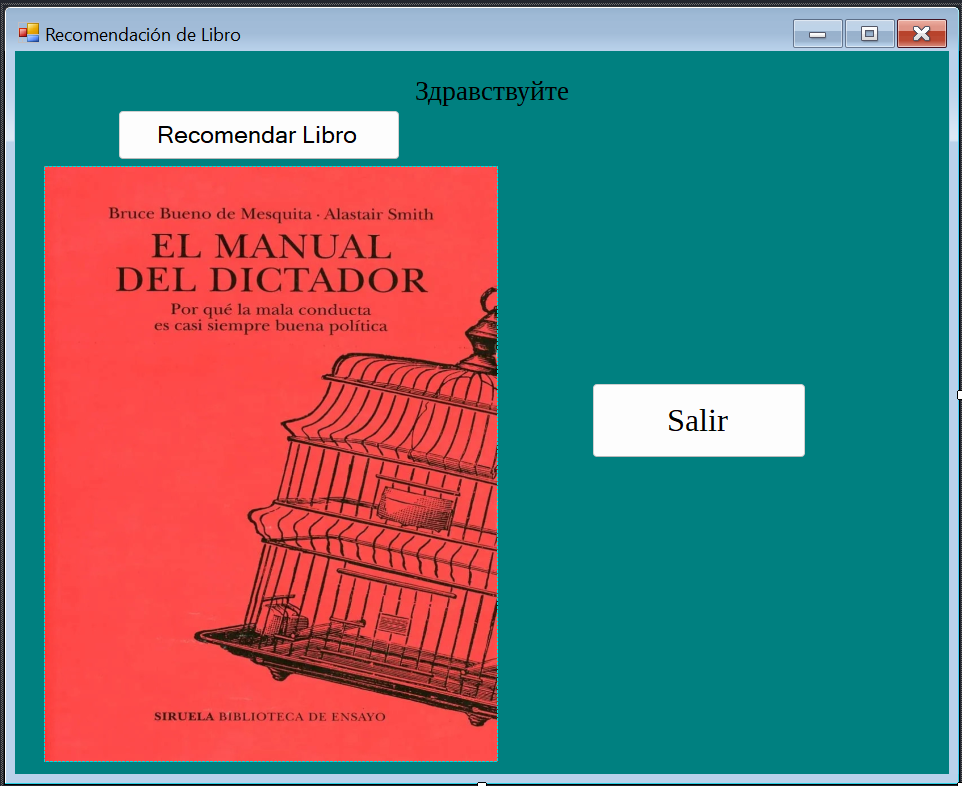
\includegraphics[scale = 0.4]{Imagenes/ui_2.png}
  \caption{Form 2}{Fuente: Propia}
\end{figure}
\subsection{Código del programa}
\lstinputlisting[style=vbstyle]{Codigo/codigo_menustrip.vb}
\chapter{Conclusiones}
El MenuStrip en Visual Studio es una poderosa herramienta que permite a los desarrolladores implementar menús intuitivos y estructurados en aplicaciones de escritorio. Su flexibilidad y facilidad de uso no solo agilizan el desarrollo, sino que también optimizan la interacción del usuario con la aplicación. Su correcta implementación permite un acceso rápido y eficiente a las funcionalidades clave del software, mejorando significativamente la usabilidad y la organización de los comandos.
\chapter{Consideraciones Finales}
Desde mi experiencia trabajando con MenuStrip en Visual Studio, puedo decir que es una herramienta bastante versátil y fácil de implementar en proyectos de aplicaciones de escritorio. Su capacidad para organizar y presentar comandos de manera clara en un menú desplegable facilita mucho la navegación dentro de la aplicación. A nivel de desarrollo, me resultó intuitivo crear menús jerárquicos y asignarles atajos de teclado, lo que me permitió mejorar la usabilidad de la interfaz. Sin embargo, creo que requiere cierta planificación previa para estructurar bien los menús y evitar sobrecargar al usuario con demasiadas opciones. En general, considero que el MenuStrip es fundamental para desarrollar aplicaciones más organizadas y profesionales.
\end{document}